\section{Proposed method}
\label{sec:method}

In this work, we investigate the profound contribution of attention mechanism to grasp detection area. Based on the recent successful end-to-end model VoteGrasp (\textcolor{cyan}{\cite{hoang2022context}}), we examine a set of attention modules by integrating each of them into VoteGrasp. In this way, we convey insights about their essence to grasp detection as well as their operations. Concretely, the architecture of our proposal will be clarified in \ref{sec:vote_grasp} and the attention modules will be deeply discussed in \ref{sec:attentions}.

\subsection{VoteGrasp}
\label{sec:vote_grasp}

\begin{figure*}[h!]
	\centering
	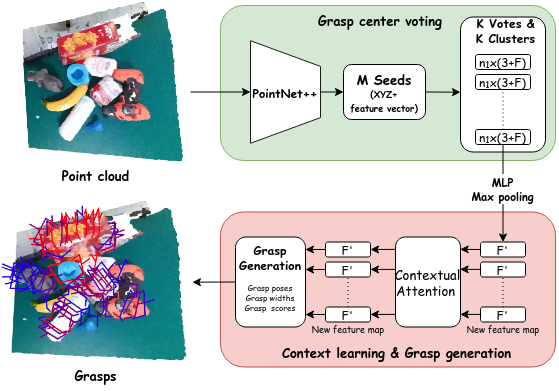
\includegraphics[width=0.8\linewidth]{figs/VoteGrasp.png}	
	\caption{VoteGrasp model using voting architecture and attention module for 6-DOF grasp detection in point cloud data. Our model conducts several self-attention modules discussed in section \ref{sec:attentions} following Hough voting network (\textcolor{cyan}{\cite{qi2019deep}}) to learn contextual information. Green grasps refer to highest quality grasps and red ones refer to lowest quality grasps.}
	\label{fig:VoteGrasp}
\end{figure*}

VoteGrasp is designed based on voting mechanism to overcome the obstacle of detecting grasps in occlusion and cluttered environments. Fig.\ref{fig:VoteGrasp} illustrates the overall architecture of VoteGrasp. Given a point cloud input of size $N\times3$, our method outputs a set of potential grasps, in which each grasp $G=(p,R,w,q)$ is accompanied by a center point $p=(x, y, z) \in \mathbb{R}^3$, gripper orientation $R \in SO(3)$, gripper width $w \in \mathbb{R}$, and grasp score $q \in [0,1]$. In terms of gripper estimation, we reformulate $R$ as in (\textcolor{cyan}{\cite{kehl2017ssd}}) instead of directly regressing it because of non-linearlity of the rotation space (\textcolor{cyan}{\cite{peng2019pvnet}}). 

\textbf{Backbone Network:} We take advantage of PointNet++ architecture as our backbone to extract geometric features. PointNet++ consists of set learning layers to combine features from multiple scales therefore able to enrich local features with increasing contextual scales. This backbone network prefers $M$ seed points and extracts high-dimensional features $\lbrace{s_i}\rbrace^{M}_{i=1}$ where $s_i=[x_i,f_i]$ is feature of a seed point specified by seed location in 3D space $x_i \in \mathbb{R}^{3}$ and feature vector $f_i \in \mathbb{R}^{F}$.

\textbf{Vote and Cluster:} The $M$ seed points are used as materials for computing votes for grasps. Each vote is characterized by a grasp center point and a feature vector for learning grasp. To obtain this, a multi-layer perceptron (MLP) containing fully connected layers, ReLU, and batch normalization is employed to compute $J$ votes per seed. This allows us to estimate multiple grasp poses for each object. We collect a set of votes $\lbrace \lbrace v_{ij} = [y_{ij}, g_{ij}] \in \mathbb{R}^{3+F}\rbrace^{M}_{i=1}\rbrace^{J}_{j=1}$. Here $v_{ij}$ is $j^{th}$ vote in $J$ set votes at $i^{th}$ point in $M$ seed points. $y_{ij}$ and $g_{ij}$ ($F$-dimensions) represent grasp center and feature vector learned for final grasp detection of vote $v_{ij}$ correspondingly. The next vital step is to cluster the votes by uniform sampling and finding neighboring votes within a certain Eclidean distance. Basing on a grasp center ${y_i}$ from a vote $\lbrace v_i=[y_i,g_i] \in \mathbb{R}^{3+F} \rbrace^{M \times J}_{i=1}$ calculated in previous step, we use iterative farthest point sampling (FPS) to select a subset of $K$ votes $\lbrace v_{ik} \rbrace^K_{k=1}$ in the neighborhood. A ball query finds $K$ neighboring votes $v_{ik}$ within a radius vacinity. The output are $K$ groups of vote sets of size $K \times n_k \times (3+F)$, where each group elects a grasp center and $n_k$ is number of neighbors of vote $v_{ik}$.

\textbf{Context learning:} In cluttered environments, grasping is inherently challenging because a successfull grasp has to be aware of both invisible object parts and potential collisions. The relationships between objects in the scene play an essential role in detecting collision-free grasps. Therefore, the correlations between objects and contextual information outside of interest regions are encoded into features to facilize this critical information to be learned. However, VoteNet (\textcolor{cyan}{\cite{qi2019deep}}) is originally designed to detect objects independently thanks to grouping votes which respond to one object centroid. Each cluster $C_k$ is fed into MLP layers to immediately regress its object class and bounding box. In our work, instead process each cluster instantly, we compute a new feature map by attaching relationship information between all clusters. Inspired by self-attention-based models (\textcolor{cyan}{\cite{vaswani2017attention}},\textcolor{cyan}{\cite{xie2018attentional}}, \textcolor{cyan}{\cite{wang2018non}}, \textcolor{cyan}{\cite{fu2019dual}}), we integrate a contextual module into our framework to acquire interdependencies between clusters. In more detail, votes $\lbrace v_i = [y_i,g_i] \in \mathbb{R}^{3+F} \rbrace ^{n_k}_{i=1}$ in each clusters $K$ are firstly fed into a MLP and max-pooling layer to aggregate a single feature vector $C_k \in \mathbb{R}^{F'}$. Summarizing all these single vector of $K$ clusters, we gain a feature map $C=[C_1;C_2;...;C_K] \in \mathbb{R}^{F \times F'}$. The next step is to learn correlations between clusters in $C$ by conducting a context learning module. New rich contextual feature map is generally formulated as Eq.\ref{eq:VoteGrasp_compute_context}. The particular form of formulation depends on the certain attention module applied and it is deeply discussed in \ref{sec:attentions}.
%%%%%%%%%%%%%%%%%%%%%%%%
\begin{align}
\label{eq:VoteGrasp_compute_context}
C^{context}_i = \sum_{}^{} f(\theta(C_i), \psi(C_j)) \odot g(C_j) \
\end{align}
%%%%%%%%%%%%%%%%%%%%%%%%
Where $\theta(.)$, $\psi(.)$, $g(.)$ are learnable transformations and $f(i)$ is relation function to encode relation between all positions. The widespread relation function is the dot-product family, but in our research, we further examine other relation functions. The new feature map $C_{context} = [C^{context}_1; C^{context}_2;...;C^{context}_K \in \mathbb{R}^{K \times K'}$ has same size with input feature. By leveraging self-attention mechanism, our network enables features of different clusters to communicate with each other. The contribution and effectiveness of the context learning module will be thoroughly illustrated in later sections.

\textbf{Grasp Detection:} New feature map $C^{context}$, which is enlarged with relationships between clusters, is then passed through a multi-layer perceptron (MLP) network to detect a ranked list of grasps $G=(p,R,w,q)$. More specifically, our model detects a grasp center $p=(x,y,z) \in \mathbb{R}^3$, gripper orrientation $R \in SO(3)$, gripper width $w \in \mathbb{R}$, and grasp quality $q \in [0,1]$. The MLP is implemented with 3 fully connected layers and two first of them are followed by batch normalization and ReLU. The last one - the prediction layer has $5+V+2A$ channels, in particular they are 3 grasp center regression values, 1 gripper width regression value, 1 grasp cinfidence regression value, $V$ viewpoint scores, $A$ angle scores (in-plane rotation), and $A$ angle residual regression values (in-plane rotation). $V$ and $A$ represent the numbers of sampled viewpoints and in-plane rotations respectively.

\textbf{Loss Function:} The grasp detecton is supervised with multi-task loss:
%%%%%%%%%%%%%%%%%%%%%
\begin{align}
L_{votegrasp} = L_{vote} + L_{grasp} \
\end{align}
%%%%%%%%%%%%%%%%%%%%%
The VoteGrasp loss $L_{votegrasp}$ includes a voting loss $L_{vote}$ and a grasp estimation loss $L_{grasp}$. Voting loss is built as a regression loss:
%%%%%%%%%%%%%%%%%%%%%
\begin{align}
L_{vote} = \frac{1}{M_s} \sum_{i}^{} {\lVert y_i-c^g_i \rVert}_H \cdot \mathds{1}(x_i)   \
\end{align}
%%%%%%%%%%%%%%%%%%%%%
Where $M_s$ denotes the total number of seeds on the object surface, $c^g_i$ is the closest ground truth grasp center, ${\lVert \cdot \rVert}_H$ is the Huber norm and $\mathds{1}(\cdot)$ is a binary function that indicates whether or not a seed point $s_i$ belongs to an object. In terms of grasp loss function, it is defined as follows: 
%%%%%%%%%%%%%%%%%%%%%
\begin{align}
L_{grasp} = L_center + \alpha L_{rot} + \beta L_{width} + \gamma L_{score} \
\end{align}
%%%%%%%%%%%%%%%%%%%%%
The grasp loss consists of a grasp center loss (regression) $L_{center}$, a rotation loss $L_{rot}$, a gripper width loss (regression) $L_{width}$, and a grasp confidence score (regression) $L_{score}$. The grasp center loss is conducted with two elements $L_{center} = L_{viewpoint} + L_{in-plane}$. While $L_{viewpoint}$ represents for viewpoint classification, the in-plane rotation estimation is designed as a combination of classification and regression as $L_{in-plane} = 0.1L_{angle-cls}+L_{angle-reg}$ (\textcolor{cyan}{\cite{qi2018frustum}}). We conduct $L1$-smooth loss (\textcolor{cyan}{\cite{ren2015faster}}) for all regression ingredients and standard cross entropy for classification losses. 

\vspace{0.2cm}

\subsection{Attentions}
\label{sec:attentions}
In this section, we want to thoroughly discuss attention modules that we employ in our research. This provides insights into how attention mechanism operates in each module and its potentiality in collision-free grasp detection. We will examine how differently they capture interdependencies inside feature map and operate relation function. The detail of implementation and results of plugging each module into VoteGrasp are evaluated in section 4.
%%%%%%%%%%%%%%%%%%%%%%%%%%%%%%%%%%%%%%%%%%%%%%%%%%%%%%%%%%%%%%%%%%%%%%%%%%%%%%

\textbf{Non-local} (\textcolor{cyan}{\cite{wang2018non}}):
The idea of this method is inspired by non-local means algorithm (\textcolor{cyan}{\cite{buades2005non}}) for denoising images. Non-local means computes the denoised value at a position as a weighted average of all pixels in the image. The family of weights between two pixels depends on the similarity between them. Non-local Neural Network forms this idea into deep stacks of convolutional operations to capture long-range dependencies in sequential data. 
%%%%%%%%%%%%
\begin{gather}
	\label{eq: non_local_comp_response}
	y_i = \frac{1}{C(x')} \sum_{\forall j}^{} f(x_i, x'_j)g(x'_j) \\
	\label{eq: non_local_comp_z}
	z_i = W_z y_i + x_i \
\end{gather}

%%%%%%%%%%%%%%%%%%%%
\begin{figure}
 	\centering	
 	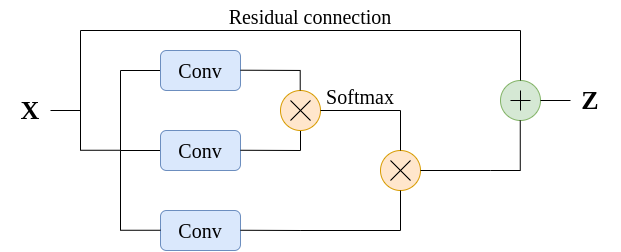
\includegraphics[width= 0.8\linewidth]{figs/non_local_diagram.png}
 	\caption{Non-local block diagram. The input feature is transformed by $1 \times 1 \times 1$ convolutions. $``\otimes"$ denotes matrix multiplication, and $``\oplus"$ denotes element-wise sum.}
 	\label{fig:non_local}
\end{figure}
%%%%%%%%%%%%%%%%%%%%

Eq.\ref{eq: non_local_comp_response} computes responses $y$ based on relationships between different locations. It is proved to be a generic non-local operation due to the fact that it takes all positions $\forall j$ into consideration. $x$ is the input signal, which could be images, videos, but often features. To reduce the computation, the authors use $x'$ as a subsampled version of $x$ by using pooling technique (max pooling). $z$ is the output feature that has variable sizes as input $x$ and therefore keeps the positional correspondences of input data to be intact. $i$ is the index of an output position and $j$ is the index that enumerates all positions. $f$ is the pairwise function (relation function) that represents the relationship between $i$ and all $j$. In this research, authors examine the use of several pairwise functions of Gaussian, Embedded Gaussian, Dot product, Concatenation, or simply done by matrix multiplication as shown in Fig.\ref{fig:non_local}. $g$ represents the input signal at position $j$. $C(x')$ is normalizing factor and softmax function is used here. The non-local operation in Eq.\ref{eq: non_local_comp_response} is wrapped into a non-local block by adding residual connection component “$+x_{i}$” as define in Eq.\ref{eq: non_local_comp_z}. This residual connection facilitates non-local block to insert a new one into the pre-trained model and does not interrupt its initial weight matrix $W_z$. This lightweight and easy-to-implemented block is plugged into many architectures such as classification, and segmentation to learn “where” they should pay more attention.

%%%%%%%%%%%%%%%%%%%%%%%%%%%%%%%%%%%%%%%%%%%%%%%%%%%%%%%%%%%%%%%%%%%%%%%%%%%%%

\textbf{Criss-cross} (\textcolor{cyan}{\cite{huang2019ccnet}}):
Similar to Non-local block, this building block is conducted to capture pixel-wise dependencies between all positions in images. Non-local block performs significantly in classification tasks. Nonetheless, confronting dense prediction tasks such as segmentation, which heavily requires high resolution of feature maps, pressures this method to reveal its weakness in consuming huge computation complexity and GPU memory. Therefore, criss-cross attention module harvests contexts in images’ criss-cross paths to obtain dense contextual information while keeping feature maps to be lightweight. In other words, this architecture prefers aggregating contextual information in horizontal and vertical directions to averaging all pixels. As a result, this is $11\times$ faster and saves $85\%$ FLOPs in comparison with non-local block. Given an input feature map $X \in \mathbb{R}^{H \times W}$, non-local produces $H \times W$ weights, while criss-cross method generates $H+W-1$ weights. However, the pixels not in a criss-cross path are still absent in the aggregation of one pixel. The authors use $(R=2)$ loops of criss-cross attention modules to guarantee full-image pixels are harvested to produce feature maps with dense contextual information. Adding this block to architectures allows them to boost their performance in both result accuracy and inference time.
%%%%%%%%
\begin{figure*}[h!]
 	\centering	
 	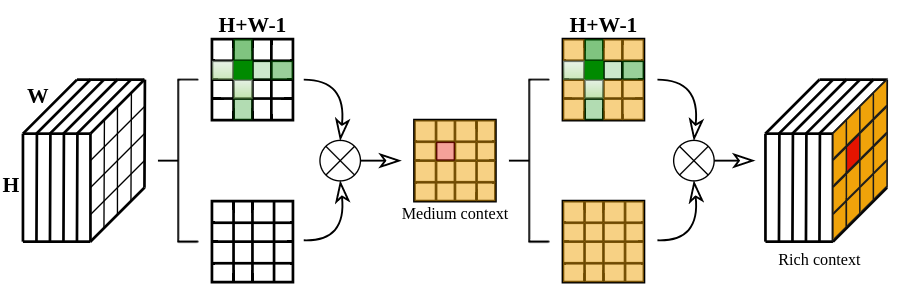
\includegraphics[width= 0.8\linewidth]{figs/criss-cross.png}
 	\caption{Criss-cross block architecture captures interdependencies in vertical and horizontal directions. The block consists of two criss-cross operations to capture interdependencies of all pixels. The differences in shades of green represent different meanings that a pixel contributes to the target pixel (red). Similarly, the differences in shades of yellow illustrate the wealth of contextual information.}
 	\label{fig:criss-cross}
\end{figure*}
%%%%%%%%

%%%%%%%%%%%%%%%%%%%%%%%%%%%%%%%%%%%%%%%%%%%%%%%%%%%%%%%%%%%%%%%%%%%%%%%%%%%%%%

\textbf{Squeeze-and-Excitation (SE)} (\textcolor{cyan}{\cite{hu2018squeeze}}):
This research strengthens the power of the convolutional operator by exploiting the interdependencies between the channels of convolutional features. Instead of focusing on spatial relationships like non-local and criss-cross network, it looks into another aspect – the relationship between channels. This block consists of two modules: Squeeze and Excitation. Squeeze operation aims to produce channel descriptors that embed global distribution feature responses. Using global average pooling allows this module to generate channel-wise statistics $y$. Given a input feature map $X \in \mathbb{R}^{H \times W \times C}$ and $x_c \in R^{H \times W}$ is the feature map at $c^{th}$ channel. A $c^{th}$ element of $y$ is calculated at $c^{th}$ channel of input data as following formula. Thus, $Y \in \mathbb{R}^C$ is a collection of average representation of all pixels of all channels.
%%%%%%%%
\begin{figure*}[h!]
 	\centering	
 	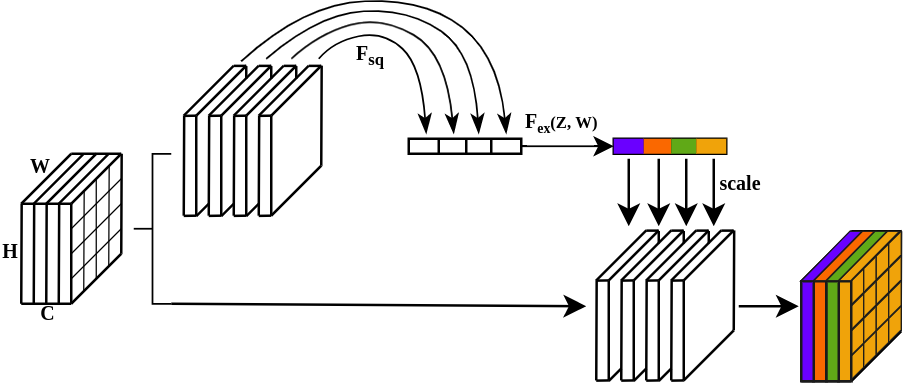
\includegraphics[width= 0.8\linewidth]{figs/SE.png}
 	\caption{Squeeze-and-Excitation block focuses on the channel relationship of input feature. Different colors depict the distribution of channel information.}
 	\label{fig:SE}
\end{figure*}
%%%%%%%%%%%%%%%%%%%
%%%%%%%%%%%%%%%%%%
\begin{gather}
\label{eq:SE_F_squeeze}
y_c = F_{sq}(x_c)= \frac{1}{H \times W}\sum_{i=1}^{H} \sum_{j=1}^{W}x_c(i,j)\\
\label{eq:SE_F_excitation}
s=F_{ex}(y, W)\\
z_c = s_c y_c \
\end{gather}

The next operation – Excitation – aggregates the information in the previous one. This one focuses on totally gathering channel-wise dependencies. To obtain this purpose, it makes use of a simple self-gating mechanism that takes embedding features, which is the output of Squeeze operation, as input to generate per-channel modulation weights $s \in \mathbb{R}^C$ as Eq.\ref{eq:SE_F_excitation}. At the end of the operation, input feature map $X$ is rescaled with modulation weight $s$. The final feature map $Z \in \mathbb{R}^{H \times W \times C}$ can indicate to what extent each channel is informative. This output map can be used by subsequent layers and help them learn “what” they should look at. This block is proved to be insertable to neural network architectures to boost their performance in scene classification and object detection.

%%%%%%%%%%%%%%%%%%%%%%%%%%%%%%%%%%%%%%%%%%%%%%%%%%%%%%%%%%%%%%%%%%%%%%%%%%%%%%%%
\textbf{Compact Generalize Non-local (CGNL) (\textcolor{cyan}{\cite{yue2018compact}})}:
This compact block is designed to achieve high accurate object recognition, especially in fine-grained objects and actions. The research notices the lack of considering interactions between positions across channels of non-local module or even criss-cross module. They solely capture dependencies between spatial pixels and temporal frames by merging channels. Hence, they pay more attention to object part relations but neglect crucial clues for recognizing actions - the interactions between objects, which correspond to different channels. Although SE network mentioned previously learns interdependencies between channels, it treats all positions in a similar way by global averaging as Eq.\ref{eq:SE_F_squeeze}. Therefore, to acquire long-range correlations as well as interactions, CGNL learns correlations among all elements across the channels by merging channels into positions. It could be clearly understood that this method fuses channel information into positional features. The input feature map $X \in \mathbb{R}^{H \times W \times C}$ is firstly divided into $G$ groups and each sub-feature map $X'$ contains $C' = C/G$ channels. In comparison with \ref{eq: non_local_comp_response}, CGNL reshapes the output of transformation function to $HWC'-D$ vector column as Eq.\ref{eq:CGNL_reshape_transform} to fuses channel into position.
%%%%%%%%%%%%
\begin{gather}
\label{eq:CGNL_reshape_transform}
\theta(X') = vec(X'W_{\theta}) \in \mathbb{R}^{HWC'} 	\\
\phi(X') = vec(X'W_{\phi}) \in \mathbb{R}^{HWC'}		\\
g(X') = vec(X'W_g) \in \mathbb{R}^{HWC'}				\\
\label{eq:CGNL_compute_response}
vec(Y') = f(\theta(X'), \phi(X'))g(X') \
\end{gather}
%%%%%%%%%%%%%
Pairwise function (relation function) $f:\mathbb{R}^{HWC'}\times\mathbb{R}^{HWC'} \rightarrow \mathbb{R}^{HWC'}\times\mathbb{R}^{HWC'}$ can distinguish pairs of same location but at different channels so that can enrich greatly feature map for action recognizing or fine-grained object classification. Each feature map $Y'$ computed from each group is then concatenated along the channel dimension to restore $Y$. By informing this formulation, this module produces competitive or state-of-the-art result on benchmark datasets.

%%%%%%%%%%%%%%%%%%%%%%%%%%%%%%%%%%%%%%%%%%%%%%%%%%%%%%%%%%%%%%%%%%%%%%%%%%%%%%%
\textbf{Dual Attention Network (DANet)} (\textcolor{cyan}{\cite{fu2019dual}}):
Methods discussed above solely use either position attention or channel attention. While position attention selectively calculates the feature of each pixel by a weighted average of all pixels, channel attention selectively emphasizes interdependencies between channels among all channel maps. Despite the fact that dual attention network further improves the discriminative representation of feature map by applying self-attention mechanism for both positional and channel dependencies. To obtain this, it feeds input data through two parallel modules of position attention and channel attention to capture long-range contextual information. The attention module commonly operates as the attentional component in previously reviewed methods. In the research, the authors examine the contribution of each attention module to the precise segmentation results. They perceive that the absence of any module would harm the accuracy of prediction task. Using both modules outcome highest Mean IoU indicator in scene segmentation among applying none, solely position, or solely channel attention. It could be interpreted that dual attention network allows architectures to emphasize “where” and “what” to be most meaningful. 
%%%%%%%%%%%%%%%%%%%%%%%%%%%%%%
\begin{figure*}[h!]
	\centering
	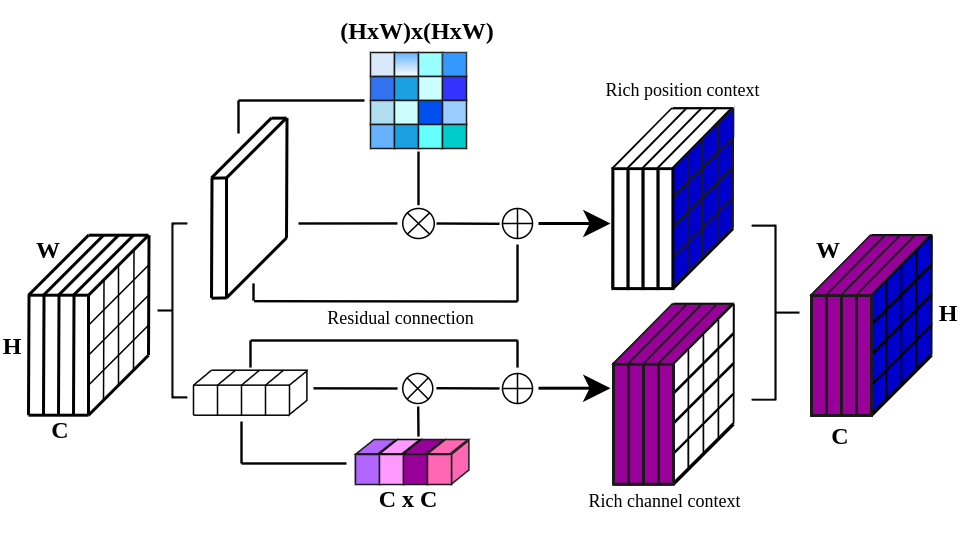
\includegraphics[width = 0.65\linewidth]{figs/Dual_attention.png}
	\label{fig:Dual_attention}
	\caption{Architecture of dual attention network includes two module of position attention and channel attention. The output feature is rich of position context and channel context.}
\end{figure*}

%%%%%%%%%%%%%%%%%%%%%%%%%%%%%%%%%%%%%%%%%%%%%%%%%%%%%%%%%%%%%%%%%%%%%%%%%%%%%%
\textbf{Convolutional Block Attention Module (CBAM)} (\textcolor{cyan}{\cite{woo2018cbam}}):
Similar to DANet for upgrading discriminative features, this module employs both spatial and channel information for attention mechanism. However, this one is different from DANet that it conducts spatial and channel attention modules in a sequential arrangement. Research also investigates diverse combinations of these two attention modules: placing the channel module first, placing the spatial module first, placing them in parallel, and placing them in sequence. Practical experiments reveal that organizing the spatial module following up channel module achieves the lowest error rate. Moreover, plugging into pre-existing architecture such as MobileNet, Faster-RCNN, StairNet, SSD, and CBAM reach slight successful detection in comparison with Squeeze-and-Excitation block.

%%%%%%%%%%%%%%%%%%%%%%%%%%%%%%%%%%%%%%%%%%%%%%%%%%%%%%%%%%%%%%%%%%%%%%%%%%%%%%
\textbf{Point-Attention} (\textcolor{cyan}{\cite{feng2020point}}):
Attention mechanism obviously demonstrates its strength in upgrading the performance of prediction architectures. However, most of them are being used for 2D data due to applying for 3D data is not straightforward. 3D point clouds inherently are irregular, sparse, unordered, and non-grid structures. Immediately exploiting the above methods for 3D point clouds might require voxelization which losses informative components of input data. Information about neighbors is crucial in attention operation so that the process of converting point clouds into a discrete grid appears to be destructive to final results. Therefore, Point Attention Network (PAN) is introduced to employ self-attention mechanism while directly dealing with 3D point clouds. It captures neighbors’ contextual correlation in multi-directions to enrich local shape features by layers called Local Attention-Edge Convolution (LAE-Conv). Then, the following point-wise spatial attention module obtains long-range spatial contextual dependencies to achieve more precise segmentation. In 3D point set, some points far away from a particular point pi appear to be not meaningful to the representation of $p_i$. Therefore, PAN conducts LAE-Conv to search for meaningful neighbors beforehand to enhance the local representation of point $p_i$. A ball space of a central point with $r$ radius is formed and divided into $K$ uniform bins. Radius $r$ is selected to ensure that each bin contains at least $m$ neighbors and only $m$ nearest neighbors contribute to the representation of the central point. Experiments yield $K=16$ and $m=1$ gain the highest accuracy. In comparison of this searching operation with other methods, we have some clear discussion. PointNet++ searches neighbors within a ball query radius. A PointNet-based hierarchical network separately processes local points. It, however, ignores the relationships between points. Moreover, the ball query selects all points inside the ball which would be tricky if the number of neighbors is small. On the other hand, although K-nearest neighbors (KNN) outputs a fixed number of neighbors, it does not guarantee that neighboring information comes from all directions. Neighborhood points found by LAE-Conv are not treated equally, the contribution of neighbors is computed by attention mechanism and the updated features of central point $p_i$ are aggregated with respect to $K$ neighbors.
\begin{gather}
\label{eq:alpha_point_attention}
\alpha_{ij}= softmax(a(W(p_j - p_i))) \\
\label{eq:p_i_point_attention}
p'_i = \sum_{j \in N_{p_i}} \alpha_{ij} W_{p_j}\
\end{gather}

Where $p_i$ is central point and its neighbor $p_j$. $\alpha_{ij}$ is weight coefficient of point $p_j$ to contribute to $p_i$ and it is normalized by softmax function. $W$ is a learnable weight matrix that transforms the input point to a higher-level local feature. $(p_j-p_i)$ is a function to transform neighbor to local coordinate systems. $p'_i$ is the higher-level feature of central point $p_i$. The wealthy representation of local geometric features extracted from LAE-Conv is fed into Point-wise spatial module to further capture long-range contextual information. This is obtained by the prevalent attention mechanism as shown in Fig.\ref{fig:point_attention}. Weight map $S$ is computed weight function added softmax normalization. The presence of PLAE in Fig.\ref{fig:point_attention} refers to residual connection. Practicing PAN on challenging benchmarks proves its ability to achieve 3D object detection is competitive with other state-of-the-art methods.
%%%%%%%%%
\begin{figure*}[h!]
\centering
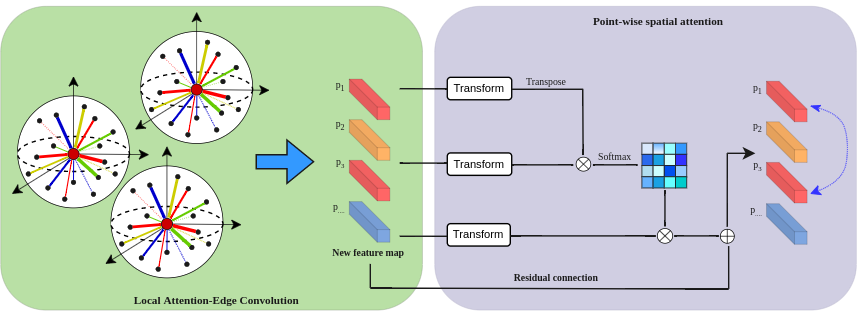
\includegraphics[width= \linewidth]{figs/Point_attention.png}
\caption{Local-global architecture of Point-attention block contains Local Attention-Edge Convolution module and Point-wise spatial attention. The first module searches a target point's 16 neighbors within a ball and computes a new feature map, which is enriched with geometric information of neighbors. The thickness of lines connecting the center point to neighbors refers to different contributing values. After enlarging local representation, the second module captures global correlations.}
\label{fig:point_attention}
\end{figure*}

%%%%%%%%%%%%%%%%%%%%%%%%%%%%%%%%%%%%%%%%%%%%%%%%%%%%%%%%%%%%%%%%%%%%%%%%%%%%%%
\textbf{Point Transformer} (\textcolor{cyan}{\cite{zhao2021point}}):
A self-attention-based backbone for diverse tasks with 3D point clouds such as object classification, object part segmentation, and semantic segmentation. The research explores the performance of two type of attention operation: scalar attention (\textcolor{cyan}{\cite{vaswani2017attention}}) and vector attention (\textcolor{cyan}{\cite{zhao2020exploring}}) and adding position encoding element as well. The attention layer of this method can be represented as follow.
%%%%%%
\begin{align}
\label{eq: point_transformer}
y_i= \sum^{}{} \rho(\gamma(f(x_i, x_j) +\varepsilon) \odot (g(x_j) +\varepsilon)) \
\end{align}
%%%%
Where $y_i$ is responses based on different locations, $\rho$ is the normalizing function, $\gamma$ is the mapping function to transform the output of the relation function to right dimensionality, and $\varepsilon$ is the position encoding element. To clearly understand the examining scalar attention and vector attention, we look closer into relation function $f$. There are two forms of attention operator: pairwise self-attention and patchwise self-attention. 
\begin{itemize}
	\item The more common pairwise self-attention, in which weight computation $f(x_i,x_j)$ is computed by aggregating all feature vectors of positions $x_i, x_j$ within whole image as Eq.\ref{eq: point_transformer}(without $\gamma$ and $\varepsilon$ ingredients). The dimensionality of relation function output depends on the form of relation function $f$. The pre-dominant formulation is dot-product attention that produces output with dimensionality equals to 1. This construction shares its output across all channels and does not adapt the attention weights at different channels. The specific choice of dot-product is termed scalar attention. The other cases of relation function such as summation, subtraction, and Hadamard production produce vector output (\textcolor{cyan}{\cite{zhao2020exploring}}) can be additionally processed to map right dimensionality to input features by $\gamma$ function. Therefore, vector weights can vary along the channel dimensions, and it is termed vector attention. In Point Transformer, subtraction relation is selected for relation function to apply vector attention. Experiments yield that using vector attention (Subtraction relation) outperforms using scalar attention (Dot-product relation). 
%%%%%%%%%%%%%%%%%%%%%%%%%%%%%%%%%%%%%%
\begin{align}
\alpha(x_i,x_j)=\gamma(f(x_i, x_j))													\\
\textbf{Dot-product:} \; f(x_i, x_j) = \varphi(x_i)^{\top} \psi(x_j) 			\\
\textbf{Summation:} \; f(x_i,x_j) = \varphi(x_i) + \psi(x_j) 				\\
\textbf{Subtraction:} \; f(x_i,x_j) = \varphi(x_i) - \psi(x_j) 				\\
\textbf{Hadamard product:} \; f(x_i,x_j) = \varphi(x_i) \odot \psi(x_j) 			\
\end{align}
%%%%%%%%%%%%%%%%%%%%%%%%%%%%%%%%%%%%
	\item Another form of attention is patchwise attention, in which the input of relation function is the patch of feature vectors $x_{R(i)}$ instead of feature vector $x(i)$ at a particular position. Moreover, the output of wight computation function alpha(xR(i)) is a tensor of same spatial dimensionality as the patch $x_{R(i)}$. Thus, patchwise attention inherently is vector attention. Several selections for relation function are Star-product, Clique-product, Concatenation (\textcolor{cyan}{\cite{zhao2020exploring}}).
	\item \textbf{Position encoding.} In pairwise attention, feature vectors $x(j)$ are processed independently so that the weight computation cannot leverage information from any location except for $i$ and $j$. Therefore, position encoding facilizes augmenting feature maps with position information. The importance of position encoding is examined in experiments suggest that applying relative position encoding for both attention $(f(x_i,x_j) + \varepsilon)$ and feature $(g(x_j)+\varepsilon)$ accomplishes the highest performance.
\end{itemize}
